\section{Background}\label{background}

This chapter provides context to the information discussed throughout the thesis and is accomplished by providing theories, concepts, terms as well as historical data from relevant studies.

\textit{Verifying Programs Using Tests} describes two testing methods and some of their limitations as well as what a test-driven development (TDD) is. \textit{Verifying Programs Using Tests} also has a description of the concept of property-based testing. \textit{Formal Specification} provides a description of what the purpose of the technique is and how it has been used in the field of software development. It also contains a description of TLA+ which is the formal specification language used during this project. The sections \textit{C}, \textit{Rust} and \textit{Hoare Logic} provides background information about those topics and \textit{FreeBSD Linked List} describes the porting target source code and why it was chosen.






\subsection{Verifying Programs Using Tests}\label{testing}


Testing is, in general, performed in one of two ways. The first being where the functionality of the system is tested from an outside perspective without peering into its internal structure. This verifies that the expected outputs are produced on a given set of inputs and is a method usually called black-box, or functional testing. The second way of testing is where the internal structure and design of the program - its state - is being tested and is usually called white-box, or structural testing \cite{comparison}. It is not feasible through testing alone, by either of these disciplines, to guarantee the absence of bugs. It is only possible to verify that a piece of code behaves in some way given a specific, finite, set of inputs. Consider, for example, the pseudo-code in figure \ref{fig:pseudocode}.
\begin{figure}[H]
 \vspace{12pt}
\begin{verbatim}
                          
                          global signed z
                          function x(y):
                             z++           
                             y
                            
\end{verbatim}
    \caption{Pseudo-code Function}
    \label{fig:pseudocode}
\end{figure}

The function takes an argument as input and returns it without any mutation. It also applies the increment operator ++ on the global variable \textit{z}. As \textit{z} is signed, there are specific values of \textit{z} where the increment by one operator is not defined - namely the highest value that \textit{z} can take. From a black-box perspective, it could be concluded from even somewhat extensive testing, that the function behaves in a deterministic way and the rule described in figure \ref{fig:pseudoproperty} would hold.
\begin{figure}[H]
 \vspace{12pt}
\begin{verbatim}
                        [for all] numbers y     
                        x.apply(y) is y
                        
\end{verbatim}
    \caption{Pseudo-code Property}
    \label{fig:pseudoproperty}
\end{figure}

Achieving total coverage, even in this trivial example, would be time consuming since the input domain is all possible machine integers. It could also be the case that testing all of them would not necessarily find the bug since a possible undefined behavior of \textit{z} is independent of the functions input values. There are similar examples where the function would behave as intended when called in a certain application state, but potentially misbehave when the state is different, even if the input is the same each time. In the case of a more complex function which takes more input arguments making a linear search of the input space unfeasibly time-consuming. It could also be the case that even with many samples, the non-deterministic behavior of the function may not necessarily be exposed. Using metrics such as branches taken, or lines executed \cite{comparison} - common metrics for coverage - would not help in this case. 
Neither would automatically generate sets of input to be tested, so called property-based testing \cite{duregard_automating_2016}, necessarily find the problem since many consecutive calls to the function are needed (see section \ref{pbtesting}). The goal of testing thereby should be to find a reasonable set of tests that can verify the behavior for most input. They should also exercise the program's structural components thoroughly enough, no matter what is the correct, or intended behavior \cite{comparison}. 

By considering the structure of the program, it is possible to at least avoid constructing a set of tests which are guaranteed to be insufficient. The reasoning behind this is that it most certainly cannot be made any inference about the effects of a line of code if the line is never executed. Instead of doing an exhaustive search of the input space, structural tests give as good a guarantee that the code is covered, but with fewer test-cases. This is accomplished by basing the tests on the control structure of the program \cite{comparison} - in other words white-box testing. Tests written using the program's structural properties as a basis for test completeness should therefore be able to ascertain the behavior of the program to a degree sufficient for a starting point from which a mathematical description, or formal specification, can be created.

\subsubsection{Property-based Testing}\label{pbtesting}
Property-based testing is a way of using test-cases, not to check specific concrete cases, but rather as rules which describe some property of a function. The principle of property testing is described in \textit{QuickCheck} by K. Claessen and J. Hughes \cite{QUICKCHECK}. It entails that the test code describes some operation that is permissible unto the system under test along with the constraints on the input data for that operation. Along with the operation, some \textit{properties} such as pre- and post-conditions that must always hold true are defined. Usually this is done by the property function returning either true or false, or by using assertions. To then exercise this property, a set of concrete test-cases are automatically generated from this blue-print. The input data is usually generated according to some heuristic that is likely to find edge cases, e.g., "empty" style inputs, or inputs close to the perimeters of the range \cite{duregard_automating_2016}. This allows for a huge breadth of input parameters to be tested with very little effort.

There exists a subset of property-based testing, herein called stateful property-based testing. The purpose of this type of testing is to verify that properties of the system hold true, even over the lifetime of the system. To verify this, a model is defined. The model will usually be a simplified - but correct - version of the system under test (SUT). The model is used, before or after each operation, to verify some fact about the state of the SUT. For each operation on the SUT, a corresponding operation on the model is defined along with predicates that determine when the operation is valid. These operations can then be applied consecutively in different orders to find inconsistencies between the model and the SUT. Some testing frameworks will as an addition to finding the sequences of operations which yield inconsistencies, have some heuristic with which these sequences can be reduced to shorter ones \cite{QUICKCHECK}.

\subsubsection{Test Driven Development}

TDD is a common software development practice where tests are written first, and code is written only to satisfy these tests which initially should be failing \cite{TESTDRIVEN}. This leads to an incremental development process where development and testing is interleaved. One benefit to this process mentioned in \cite{sommerville_software_2011} is that it gives clarity to the intentions of the author - the tests make assumptions about how the code should behave explicitly. It is argued that because of this, tests make the code self-documenting. The fundamental process of TDD is an incremental, iterative one where implementation and refactoring is repeated until the tests pass \cite{sommerville_software_2011} (see figure \ref{fig:testdriven}).

\begin{figure}[H]
 \vspace{12pt}
\centerline{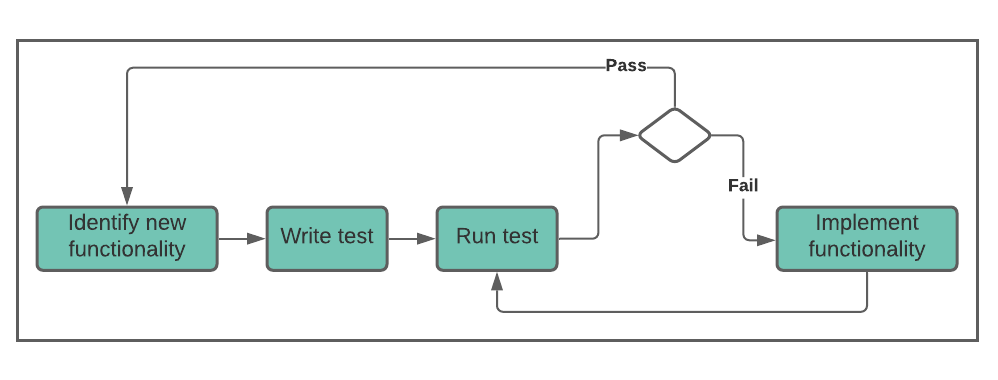
\includegraphics[width=4.8in]{TestDriven.png}}
\caption{The TDD Process}
\label{fig:testdriven}
\end{figure}

\subsection{Hoare Logic}\label{hoare}

Hoare logic is a formal system with a set of axioms and logical rules used in proofs of properties of computer programs \cite{HOARE}. Its central feature is the Hoare triple (see figure \ref{fig:hoaretriple}).

\begin{figure}[H]
 \vspace{12pt}
\begin{displaymath}
            P\{Q\}R   
\end{displaymath}
\caption{Hoare Triple}
\label{fig:hoaretriple}
\end{figure}

                        
This triple describes how the execution of a piece of code changes the state of the computation and should be interpreted as “if the assertion P is true before initiation of a program Q, then the assertion R will be true on its completion”. The use of this deductive reasoning is intended to provide a fundamental understanding of the code. 

\subsection{Formal Specification}\label{formalspec}


Building a software system is almost entirely a design activity consisting of combining, inventing, and planning the implementation of abstractions. The goal with this is to describe a set of modules interacting with one another in simple, well defined ways \cite{Larch}. If this goal is achieved it will enable engineers to work on different modules independently, while still accomplishing their common purpose. A good design will also make maintaining the software, as well as modifying its modules, easier without causing unintended effects. In summation, the key to good software design is inventing appropriate abstractions around which to structure the system.


Formal specifications are mathematically based techniques used to help with designing systems and software. Formal in this case means that they have a specific syntax, the domain of the semantics has a distinct set of meanings, and they can be used to infer useful information \cite{FORMALSPECROADMAP}. This enables them to demonstrate that a system is correct with respect to its specification while simultaneously describing system abstractions. This is accomplished independent of any of its implementations - specifications describe what a system should do, not how it should do it. This enables designers to focus attention on possible inconsistencies, deficiencies, and ambiguities leading to many mistakes and subtle bugs from many sources cropping up in specifications before they do in the implementation. This benefit could be derived from the fact that engineers focus on the safety and liveness properties of a system when using formal specifications; they need to state what needs to go right instead of focusing on what could go wrong, often a mind set when writing tests \cite{AMAZONFORMALSPEC}. Formal specifications encourage this way of thinking by describing an algorithm as a state machine, enabling a designer to create a simple and powerful abstraction of it.

\phantomsection
\label{benefits}
Since computer systems become increasingly more powerful and complex as time passes, the need for better techniques to assist in the design and implementation of reliable software becomes more prominent. Formal specifications have been around since the early days of computers and have been adopted in more traditional engineering disciplines but are not widely used in industrial software development \cite{sommerville_software_2011}. One of the reasons for this is that the method, by many, is not considered to be cost-effective. There has also been very little interaction between the test and formal specification communities, but some argue that the approaches could be used as complementary to each other for a better result \cite{USINGFORMALSPECTESTING}. 

Recent studies have also found that creating a mathematical model of a system under development led them to find and handle undesired behavior during the system analysis phase \cite{APPLYINGFORMALSPEC} \cite{AMAZONFORMALSPEC}. These studies claim that the time spent making mathematical models was well invested since it reduced the amount of time spent finding and fixing bugs during the implementation phase. This is most likely the case, since a model with good system-invariants helps engineers get the design right from the outset. The invariants capture the fundamental reason why the system works by using them as safety properties; properties that need to hold true for each possible state that the system can take. Therefore, they show that the design is not broken, which helps engineers get the code right faster since a broken design will lead to broken software - even if the code passes tests based on the design.
\\
\\
\\
Formal specifications due to its mathematical nature, however, are not an all-purpose tool. The consensus seems to be that they are most likely to be useful in data modeling where data definitions are written in a common, implementation-independent manner which lets the information pass through various development phases without transformation  This means that formal specifications are considered useful in situations such as when \cite{APPLYINGFORMALSPEC}:

\begin{itemize}
  \item There is a complex data structure that must be handled correctly.\label{formal_spec_structuer}
  \item A precise function definition is required when a simple function is needed, but it is vital that the function is implemented correctly.
  \item Complex functionality is involved with many choices to be made or many exceptional conditions arise.
\end{itemize}

To know when and how to use a formal specification takes a lot of skill and experience. For example, a formal specification does not easily model the performance of a system, and some aspects of performance cannot be modelled at all \cite{AMAZONFORMALSPEC}. If applied without consideration, a formal specification could therefore lead to a sub-optimal design even in the absence of errors. A feasible way to model a system to predict the issue of prolonged severe slowdowns seems to not be known as of this day \cite{AMAZONFORMALSPEC}. This means that other techniques need to be used combined with formal specifications to mitigate that. 

\subsubsection{TLA+}\label{tla}

TLA+ is a language developed by the computer scientist Leslie Lamport \cite{LAMPORTWEB} and has been used by, for example, Amazon since 2011 as a tool to achieve correctness in sophisticated distributed systems \cite{WHYAMAZONTLA}. They evaluated TLA+ among other languages like Alloy \cite{ALLOY} and Microsoft VCC \cite{MSVCC}. All languages had their pros and cons but TLA+ turned out to be best suited for their needs.

The evaluation found that TLA+ was best for handling very large, complex, as well as subtle problems. TLA+ was claimed to accomplish this by being able to capture rich concepts simply and directly without tedious workarounds, for example when specifying dynamic sequences of many types of nested records. It was also perceived that details from complex designs can be added or removed quickly since TLA+ supports arbitrarily complicated data structures with the ability to define powerful custom operators. This means that it was easy to adjust to a suitable level of abstraction making it a good tool when diagnosing bugs and subtle errors. Another property of TLA+ highlighted was that it tended to minimize the cognitive burden on engineers and accomplishes this by using conventional terminology since it largely consists of standard discrete math and a subset of linear temporal logic. This means that TLA+ allows for the expression of temporal relations between predicates, for example that some predicate will evaluate true \textit{eventually}, or that some predicate may be true only when another evaluates to some specific value. 

\subsubsection*{TLA+ Example}

A trivial example of how TLA+ can be used can be seen in this section, and is inspired by the works of Leslie Lamport \cite{LAMPORTVIDEO}.


\begin{figure}[H]
 \vspace{12pt}
\begin{verbatim}
                        global signed z
                        main()
                           z = someNumber()
                           z = z + 1
\end{verbatim}
    \caption{Program Example}
    \label{fig:programexample}
\end{figure}

The example program (see figure \ref{fig:programexample}) has an entry point \textit{main} and a global variable \textit{z} which gets assigned an integer through a call to the function \textit{someNumber}; a function returning said integer and has no side effects. The value of \textit{z} then gets incremented by one followed by the program terminating. This process can be described with a state machine (see figure \ref{fig:simplestatemachine}) which creates a simple abstraction of the code.

\begin{figure}[H]
 \vspace{12pt}
\centerline{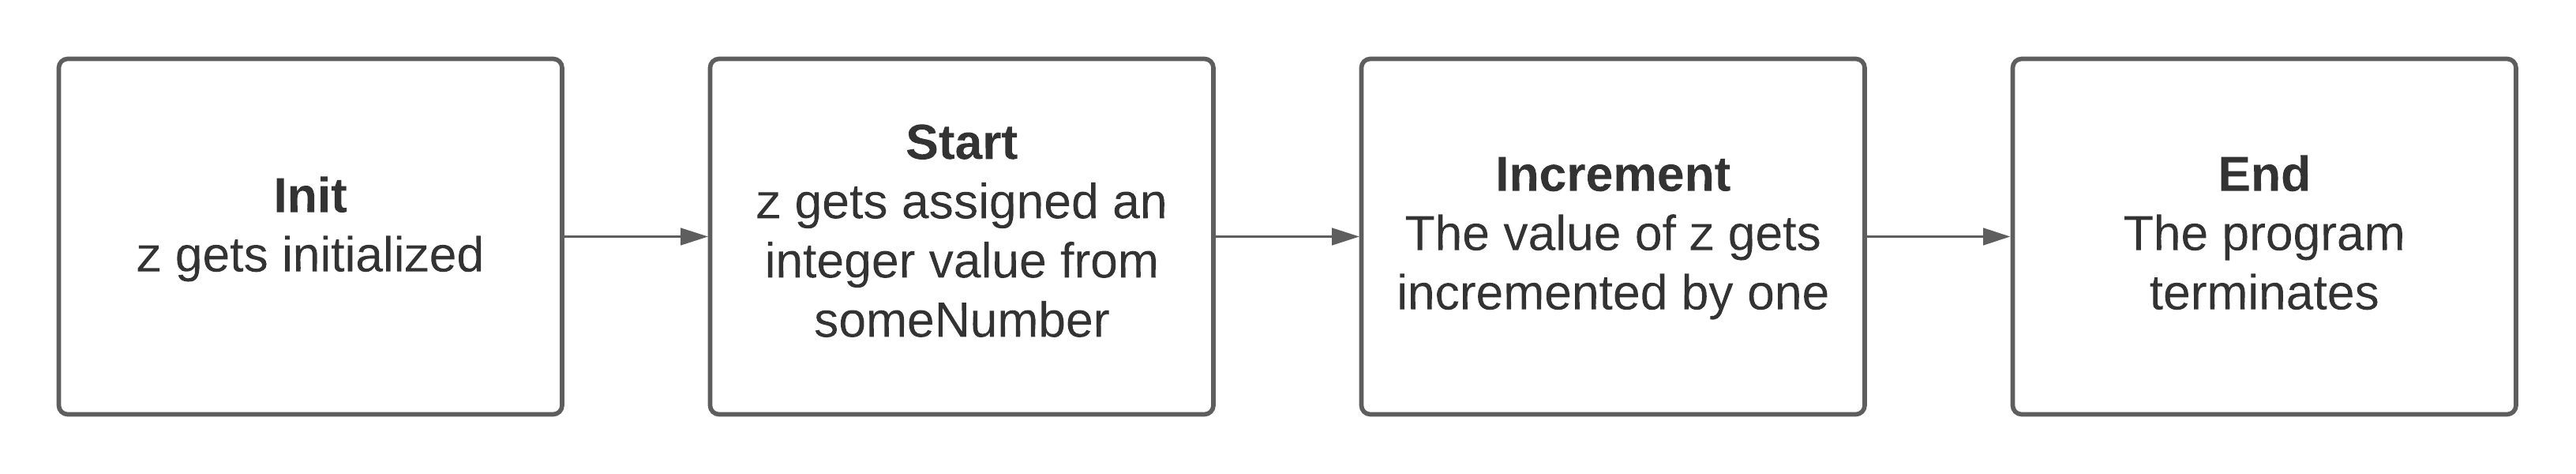
\includegraphics[width=5in, height=1in]{simplestatemachine.png}}
\caption{State Machine}
\label{fig:simplestatemachine}
\end{figure}

The state machine can then be implemented in TLA+ (see figure \ref{fig:tlaexample}). Here there is an additional variable defined called \textit{pc} which is short for program counter. It is used by the TLA+ model checker to know which state is the current one. The \textit{Init} label indicates the first state and initializes the value of the variables of the model, so the model checker knows where to begin. That the value of \textit{z} is initialized to 0 is a behavior of the language C and is used as an example but could differ depending on the language used when implementing the function. After the initializations, the model checker moves on to the label named \textit{Next} and checks which of the disjunctions (indicated by the or operator) holds true for every conjunction - in this case where the value of \textit{pc} is "start". \textit{z} then gets assigned its new value, indicated by the prime attached to it. It is accomplished by using the operator \textbackslash in which is equivalent to the mathematical operator $\in$ - member of. The function \textit{someNumber} is supposed to return any integer but TLA+ only allows for usage of finite sets. Therefore, as a compromise, \textit{z} is assigned an integer between 1 and 1000 indicated by the set operator ".." between those numbers. This means that \textit{z} becomes a member of the set of integers between one and one thousand in the current state. Lastly in this disjunction, \textit{pc} gets assigned its new value "increment". This means that the model checker moves to the state which holds true for the new value, checks it and proceeds with this practice until \textit{pc} is assigned the value “done” followed by its termination. This enables the model to be evaluated to see if every statement holds true given any situation, providing a logical foundation that the implementation does the same. If, however, it is not possible to satisfy one or more of the conjunctions, the model must be invalid, and cannot be implemented as an executable program.


\begin{figure}[H]
 \vspace{5pt}
\begin{lstlisting}
                VARIABLES z, pc

                Init == 
                    pc = "start" /\ z = 0
    
                Next == 
                    \/ /\ pc = "start"
                       /\ z' \in 1..1000
                       /\ pc' = "increment"
                    \/ /\ pc = "increment"
                       /\ z' = z + 1
                       /\ pc' = "done"
\end{lstlisting}
\caption{TLA+ Example}
\label{fig:tlaexample}
\end{figure}

\subsubsection*{TLA+ Tools}\label{tools}

The TLA+ ecosystem provides an integrated development environment (IDE) called TLA+ Toolbox \cite{TLATOOLBOX}, which allows for writing and translating the pseudo-code like language PlusCal into pure TLA+. PlusCal is a language that can express much of what TLA+ can express, but more conveniently. PlusCal even extends TLA+ with additional syntax and can be especially suitable for implementing algorithms \cite{PRACTICALTLA}.


\subsection{C}\label{c}

Since it started to gain popularity during the 1980s has the programming language C been a natural choice when programming at a low-level. Although C provides high level abstractions, nowadays C is considered a low level language due to the lack of automatic memory management and that it provides transparent, efficient access to the underlying hardware \cite{DEMYSTIFYING}. C found lasting use in applications previously coded in assembly. C provides many features not available in assembly such as several levels of scoping. This makes it possible to use the same identifier many times within a program without them necessarily interfering with each other. C also provides static type checking, meaning that type checking is performed at compile time. There are no strict rules about whether a language is strongly or weakly typed, however, since C allows the conversion of a void pointer to any other type and vice versa, it should not be considered strongly typed, Kernighan and Ritchie also consider it as such \cite{CPROGRAMMINGLANGUAGE}. 

One problem with C , especially nowadays when the alternative is not assembly language, but instead other modern programming languages, is the manual management of memory and the risks that come with this – a risk many would claim makes C an unsafe language \cite{RUSTONOMICON}. This comes from the fact that a misuse of manual memory management will cause undefined behavior. Bugs relating to mismanagement of memory can also be very hard to track down since such errors may lie dormant in the program until later when the program suddenly crashes or misbehaves. The program may also become unpredictable and create security vulnerabilities, for example when accessing some memory after the resource has already been freed (use-after-free) \cite{IMPACTOFUNDEFINED}. These problems among others have prompted the development of so-called safe languages \cite{JAVAWHITEPAPER}, many of which achieve safety through moving memory management into a layer not directly accessible to the programmer. This extra layer of virtualization - like most things - has an impact on the performance of the program often caused in large part by the garbage collector which must keep track of all allocated objects in real-time and reclaim them when they are no longer needed \cite{CPPJAVA}. 

\subsection{Rust}\label{rust}

Rust is a modern system programming language focusing on safety, speed, and concurrency and claims to accomplish these goals without using a garbage collector. Instead, the safety is enforced by the compiler by checking under what conditions objects in memory are being accessed or mutated according to some rules about data ownership. The rules regarding aliasing in Rust are quite strict, where aliasing means when two or more variables or pointers refer to the same or overlapping regions in memory. One of the most essential rules of Rust, regarding aliasing can be summarized as follows \cite{THERUSTPROGRAMMINGLANGUAGE}:

\textit{There may be one mutable \textbf{or} N number of immutable references to an object, but never \textbf{both} at the same time (N here could be any natural number).}

This is enforced statically by Rust's static analyzer called the borrow checker. The concept of mutability is also touched upon here, and it is important to understand that every variable or reference in Rust carries with it metadata about its mutability i.e. whether it can be modified. For example, if a stack-allocated variable like an integer is mutable, the programmer is allowed to reassign it with a new value. For references, mutability determines whether it is allowed to call the referenced object's mutable methods, change its properties directly, or pass it to a function that requires a mutable reference. 

By enforcing the rules at compile-time, rather than at run-time, code written in Rust can be as fast as code written in C. Designers of Rust also claim that introducing parallelism in Rust comes at a relatively low risk, since the compiler is designed to catch classical mistakes - such as race conditions - before execution \cite{RUSTONOMICON}. Code written in Rust is also claimed to always provide type- and memory-safety and situations like dangling pointers, use after free or any other kind of undefined behavior should never have to be endured by the programmer. This allows for more aggressive optimizations since they will not accidentally introduce crashes or vulnerabilities. The purpose of Rust is to eliminate the trade-offs that have been accepted when working with C while at the same time getting comparable performance \cite{THERUSTPROGRAMMINGLANGUAGE}.

\phantomsection
\label{safe}
Rust can be thought of as a combination of two programming languages - safe and unsafe Rust. Safe Rust is a subset of Rust and often considered the \textit{true} Rust programming language. This is where all the compile-time memory and type-safety checks are applied. Sometimes, however, there will be situations where low-level memory interaction is needed. In unsafe Rust, the programmer is allowed to dereference raw pointers and use other types of operations for which the compiler cannot provide the safety guarantees present in safe Rust \cite{THERUSTPROGRAMMINGLANGUAGE}. The value of this separation is that the programmer gains the benefits of having the option to use the benefits of an unsafe language — low level control over implementation details — without most of the problems that come with trying to integrate it with a completely different safe language \cite{RUSTONOMICON}. Another benefit to this separation is that the developer limits the number of lines of code that need to be debugged, whenever such a bug appears.


\newpage
\subsection{FreeBSD Linked List}\label{frebsd}


FreeBSD is a Unix-like operating system used to power modern servers and embedded platforms \cite{FREEBSD}. FreeBSD is mainly written in C, and its large codebase has been continually developed and updated since the beginning of the 90's by a large community of individuals and organizations. The codebase can therefore be considered well established and its functionality widely tried and tested. 

The LinkedList library in FreeBSD is defined in a queue header file, containing several function-like macros for a set of queue data structures. The singly linked list is a list where the ordering is upheld by the individual links themselves; each link - or node - defines the next element of the list, commonly using of pointers. To become useful in a computer program, each node in the list normally stores some value. In C this could be some structure or literal value, or a pointer to data somewhere else in memory.

\begin{figure}[H]
\centerline{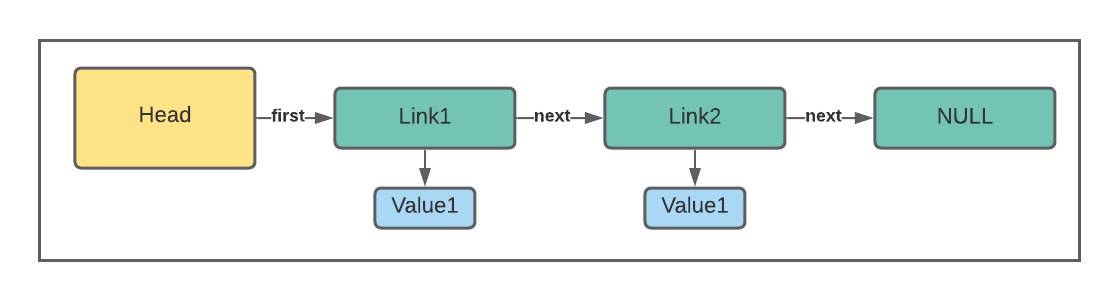
\includegraphics[width=5in]{LinkedList.png}}
\caption{FreeBSD Singly Linked List Structure}
\label{fig:freebsdlinkedlist}
\end{figure}

In the FreeBSD implementation of a singly linked list, the list consists of two structures: the head, which only contains a pointer to the first entry, and the node structure which contains some data and a pointer to the next node (see figure \ref{fig:freebsdlinkedlist}). 

\subsection{Summary}\label{motivation}

It has been shown that testing is a necessary part of software verification, but many times not sufficient for a complete understanding of a system. Property based tests with automatic test-case generation used in a white-box test discipline should maximize the utility of tests as a means of describing an existing system.

According to section \ref{formal_spec_structuer}, formal specifications can be considered most useful when handling a complex data structure. Although the complexity of a data structure is somewhat subjective, a linked list will likely contain enough complexity that the application of formalization provides some use. At the same it is common and straightforward enough that it should be understood easily by the target audience.

The properties brought up in this chapter made TLA+ a valid choice of language to use during this project. The argument is that TLA+ seems able to handle many types of problems as well as being easy be to learn. The available IDE with PlusCal support is another factor in the choice of modelling language.

If Rust manages to gain popularity and becomes ubiquitous, it is likely that it will be a target language for porting a large amount of C code in the future. Thus, the decision of using C and Rust as source and target language for this thesis seems, from the literature, as a valid and interesting choice. Using these languages will also hopefully help answering the question if formal specifications could help in getting a deeper understanding of the original system, as an intermediate step in the porting process. C and Rust, although meant to solve similar problems, have disparate design philosophies, and offer a differing feature set. This means that the linked list implementations have the potential to look vastly different. A model can describe the system without using language specific constructs, which will be important in bridging the differences of the languages.

The FreeBSD list library includes several different queues and lists. Of these, the singly linked list was chosen as the sample to port. It should to the target audience be a familiar data structure, and it is one with which the authors are well versed. Choosing a common data structure as the subject should reduce the amount of time needed to understand and describe its intricacies in greater detail.